\documentclass[]{beamer}
%\documentclass[handout]{beamer}
%\documentclass[handout,draft]{beamer}
%\documentclass[]{article}


% Preambulo
% Paquetes para usar bien el idioma español
\usepackage[spanish,es-tabla]{babel}
\selectlanguage{spanish}
\usepackage[utf8]{inputenc}

% Paquetes para usar mejores imagenes
\usepackage{graphicx}

% Paquetes para links y tabla de contenidos en el PDF
\usepackage{hyperref}
\hypersetup{colorlinks=true,allcolors=blue}
%\usepackage{hypcap}

% Paquetes para mejores tablas
\usepackage{booktabs}

% Mejor matematica
\usepackage{amsmath}

% Fuentes de las imagenes
\usepackage[absolute,overlay]{textpos}

% Paquete captions
\usepackage[justification=centering,labelformat=empty,labelsep=none]{caption}

% Opciones para ticks
\usepackage{tikz}
\usetikzlibrary{shapes,arrows,positioning}

\tikzstyle{decision} = [diamond, draw, fill=blue!20, text width=4em, text badly centered, node distance=2cm, inner sep=0pt,on grid]
\tikzstyle{block} = [rectangle, draw, fill=blue!20, text width=8em, text centered, rounded corners, minimum height=2em,on grid]
\tikzstyle{line} = [draw, -latex]

% Citas bibliograficas
\usepackage[backend=biber]{biblatex}
\renewcommand{\footnotesize}{\tiny}
\addbibresource{biblio.bib}

% Mejoro las captions
\setbeamertemplate{caption}{\raggedright\insertcaption\par}

\setbeamertemplate{caption}{%
\begin{beamercolorbox}[wd=0.85\paperwidth, sep=.2ex]{block body}\insertcaption%
\end{beamercolorbox}%
}


% Sacar barra de navegacion
\setbeamertemplate{navigation symbols}{}%remove navigation symbols

% Transparencias en items
\setbeamercovered{transparent}

% Estilo de diapositivas
% \usetheme{Boadilla}
\usecolortheme{whale}
\usecolortheme{orchid}

%\usepackage{beamerarticle}

% Titulo
\title{Herramientas de Teledetección Cuantitativa\\{\small Un viaje del sol a los píxeles}}
\author{Francisco Nemiña}

\institute{Unidad de Educación y Formación Masiva \\
Comisión Nacional de Actividades Espaciales}

\logo{
\includegraphics[height=0.7cm]{imagenes/sopi.png}}

\AtBeginSection[]
{
\begin{frame}
\frametitle{Esquema de presentación}
\tableofcontents[currentsection]
\end{frame}
}


\begin{document}
\begin{frame}
    \maketitle
\end{frame}

\section{Organización del curso}
\subsection{Objetivos, programa y cronograma}
\begin{frame}{Objetivos del curso}
  El curso tiene como objetivo\pause
  \begin{itemize}[<+->]
    \item Manejar el concepto de firma espectral.
    \item Conocer las aproximaciones realizadas al trabajar en teledetección.
    \item Corregir imágenes radiometricamente.
    \item Conocer la necesidad de dichas correcciones.
    \item Poder realizar transformaciones en el dominio espectral.
    \item Clasificar imágenes de forma supervisada y no supervisada.
    \item Validar clasificaciones de imágenes.
    \item Poder extraer valores cuantitativos en base a dicho procesamiento.
  \end{itemize}
\end{frame}
%--- Next Frame ---%

\begin{frame}{Programa}
  Vamos a dividir el curso en dos partes
  \begin{enumerate}
    \item Transformaciones en el dominio espectral.
    \begin{itemize}
      \item Firmas espectrales
      \item Correcciones radiométricas.
      \item Índices espectrales.
      \item Rotaciones en el espacio espectral.
    \end{itemize}
    \item Clasificación de imágenes en la práctica.
    \begin{itemize}
      \item Clasificaciones supervisadas.
      \item Clasificaciones no supervisadas.
      \item Técnicas de posclasificación.
    \end{itemize}
  \end{enumerate}
\end{frame}
%--- Next Frame ---%

\subsection{Aprobación del curso}
\begin{frame}{Plataforma virtual}
  \begin{block}{Urgente}
    Todo el material va a estar en
    \begin{center}
      \texttt{https://sopi.conae.gov.ar/aulavirtual}\pause
    \end{center}
    con la contraseña de matriculación
    \begin{center}
      \texttt{huethuet2017}
    \end{center}
  \end{block}\pause
  \begin{alertblock}{Importante}
    Acá se completan los cuestionarios y los trabajos prácticos.
  \end{alertblock}
\end{frame}
%--- Next Frame ---%

\begin{frame}{Notas}
  \begin{figure}
    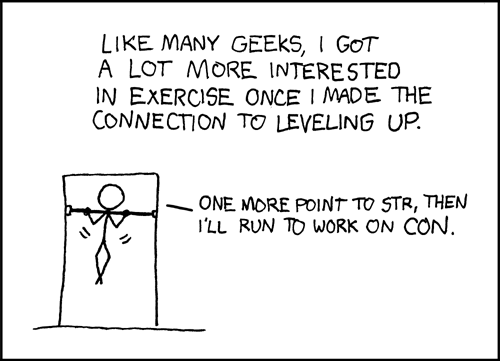
\includegraphics[width=0.6\textwidth]{imagenes/exercise.png}
    \caption{I haven't had the patience for RPGs in a long time.\footfullcite{munroe2006xkcd}}
  \end{figure}
\end{frame}
%--- Next Frame ---%

\begin{frame}{Distribución de notas}
    \begin{block}{Notas}
        \begin{itemize}[<+->]
        \item 0 - 99 - No aprobó
        \item 100-109 - Seis
        \item 110-129 - Siete
        \item 130-169 - Ocho
        \item 170-189 - Nueve
        \item 190-200 - Diez
      \end{itemize}
    \end{block}
\end{frame}
%--- Next Frame ---%

\begin{frame}{Como sumar puntos}
  \begin{itemize}[<+->]
    \item Cada cuestionario: 0 a 10 puntos. Máximo 70.
    \item Cada tarea: 0 a 50 puntos. Máximo 100.
    \item Participar en la plataforma: 0 a 10 puntos. Sin máximo.
    \begin{itemize}
      \item Hacer preguntas interesantes.
      \item Contestar preguntas.
      \item Editar artículos en la wiki.
      \item Hacer aportes.
      \item Compartir datos de campo.
      \item Encontrar la respuesta a la última pregunta sobre la vida, el universo y todo lo demás.
    \end{itemize}
  \end{itemize}
\end{frame}
%--- Next Frame ---%
\begin{frame}{Cronograma - Parte 1}
    \begin{itemize}[<+->]
    \item 26/4 - Firmas espectrales
    \item 2/5 - Entrega cuestionario 1
    \item 3/5 - Correcciones radiométricas
    \item 9/5 - Entrega cuestionario 2
    \item 10/5 - Índices
    \item 16/5 - Entrega cuestionario 3
    \item 17/5 - Rotaciones
    \item 23/5 - Entrega cuestionario 4
    \item 24/5 - Clase de consulta
    \item 30/5 - Entrega primer trabajo práctico
  \end{itemize}
\end{frame}
%--- Next Frame ---%
\begin{frame}{Cronograma - Parte 2}
    \begin{itemize}[<+->]
    \item 31/5 - Clasificaciones supervisadas
    \item 6/6 - Entrega cuestionario 5
    \item 7/6 - Clasificaciones no supervisadas
    \item 13/6 - Entrega cuestionario 6
    \item 14/6 - Técnicas de pos-clasificación
    \item 20/6 - Entrega cuestionario 7
    \item 21/6 - Clase de consulta
    \item 27/6 - Entrega segundo trabajo práctico
  \end{itemize}
\end{frame}
%--- Next Frame ---%

\begin{frame}{Área de estudio}
  \begin{block}{Definición}
    Hablaremos de teledetección cuantitativa en el espectro óptico cuando queramos obtener valores numéricos concretos a partir de la utilización de imágenes obtenidas en la región entre los $0.4\mu m$ y los $14\mu m$.
  \end{block}
\end{frame}
%--- Next Frame ---%

\section{Radiación}
\label{sec:radiacion}
\begin{frame}{Energía}
  \begin{block}{Definicíon}
    Energía es la capacidad de hacer trabajo... \pause ponele.
  \end{block}
\end{frame}
%--- Next Frame ---%

\begin{frame}{Energía}
  Es mas fácil hablar de las formas de propagación
  \begin{figure}
    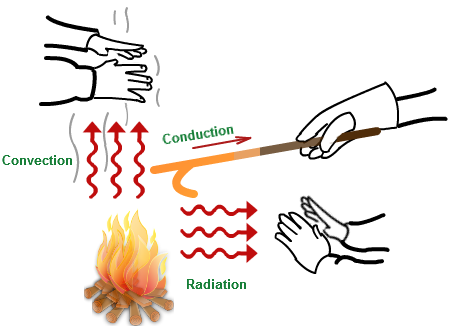
\includegraphics[width=0.6\textwidth]{imagenes/types-of-heat-transfer.png}
    \caption{Formas de transferencia de energía calor.}
  \end{figure}
\end{frame}


\begin{frame}{Energía electromagnética}
  \begin{figure}
    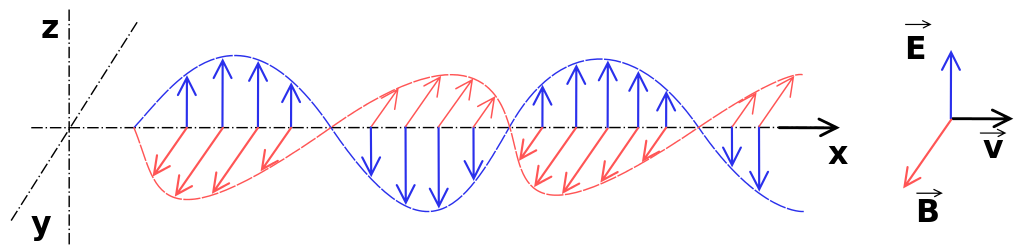
\includegraphics[width=0.6\textwidth]{imagenes/Onde_electromagnetique.png}
    \caption{De las 3, nos vas a interesar la radiación. En particular la radiación electromagnética.\footfullcite{wiki:onda}}
  \end{figure}
\end{frame}
%--- Next Frame ---%

\begin{frame}{Onda electromagnética}
  \begin{block}{Definición}
    La longitud de onda es la distancia entre dos máximos.
  \end{block}\pause
  \begin{block}{Definición}
    La frecuencia es la cantidad de oscilaciones que realiza la onda por unidad de tiempo.
  \end{block}\pause
  \begin{block}{Definición}
    La amplitud es el máximo valor posible que toma la onda.
  \end{block}
\end{frame}
%--- Next Frame ---%

\begin{frame}{Clasificación}
  \begin{figure}
    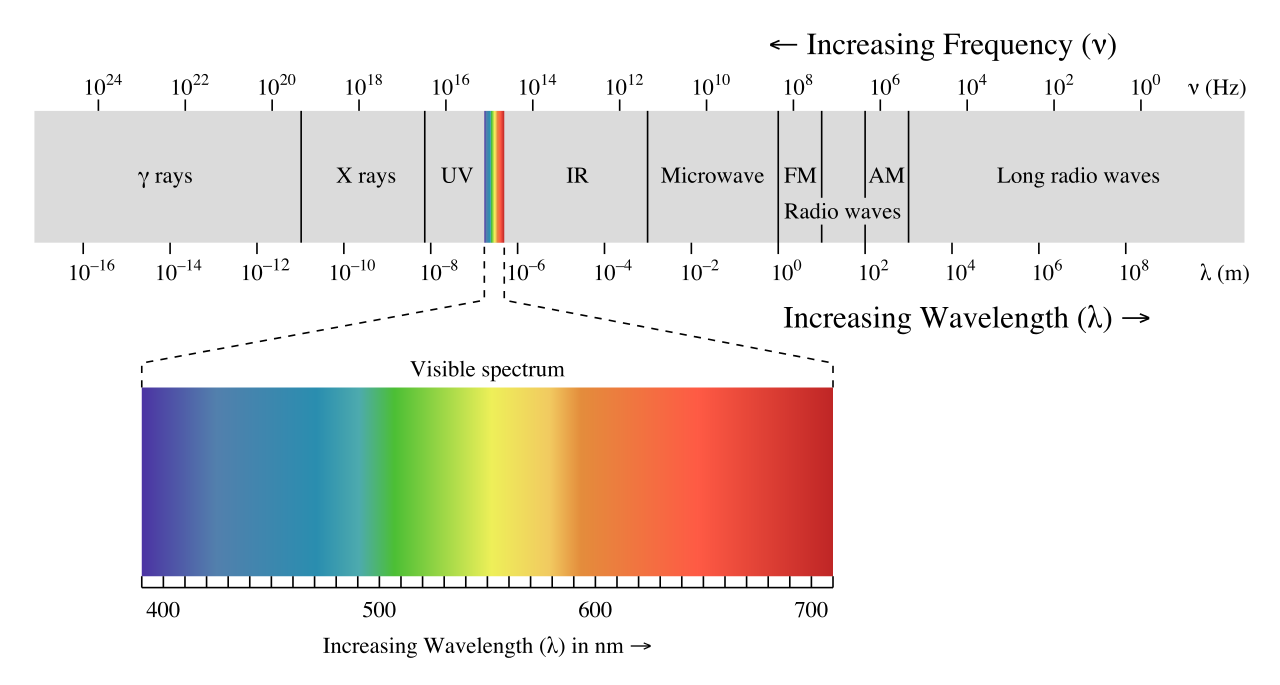
\includegraphics[width=0.8\textwidth]{imagenes/espectrum.png}
    \caption{Las ondas electromagnéticas se pueden clasificar en función de su longitud de onda en el espectro electromagnético. \footfullcite{spectrum}}
  \end{figure}
\end{frame}
%--- Next Frame ---%

\begin{frame}{Energía}
  La energía va a tener un problema como magnitud para medir porque la energía que recibo depende del tiempo en que la recibo. Veamos como mejorarlo.
\end{frame}
%--- Next Frame ---%

\begin{frame}{Potencia}
  \begin{block}{Definición}
    La potencia es la tasa de variación de energía. Es decir
    \begin{equation}
      P = \frac{\Delta E}{\Delta t}
    \end{equation}
  \end{block}
\end{frame}
%--- Next Frame ---%


\begin{frame}{Densidad de potencia}
  Veamos ahora que pasa con la potencia a medida que nos alejamos de una fuente.
  \begin{figure}
    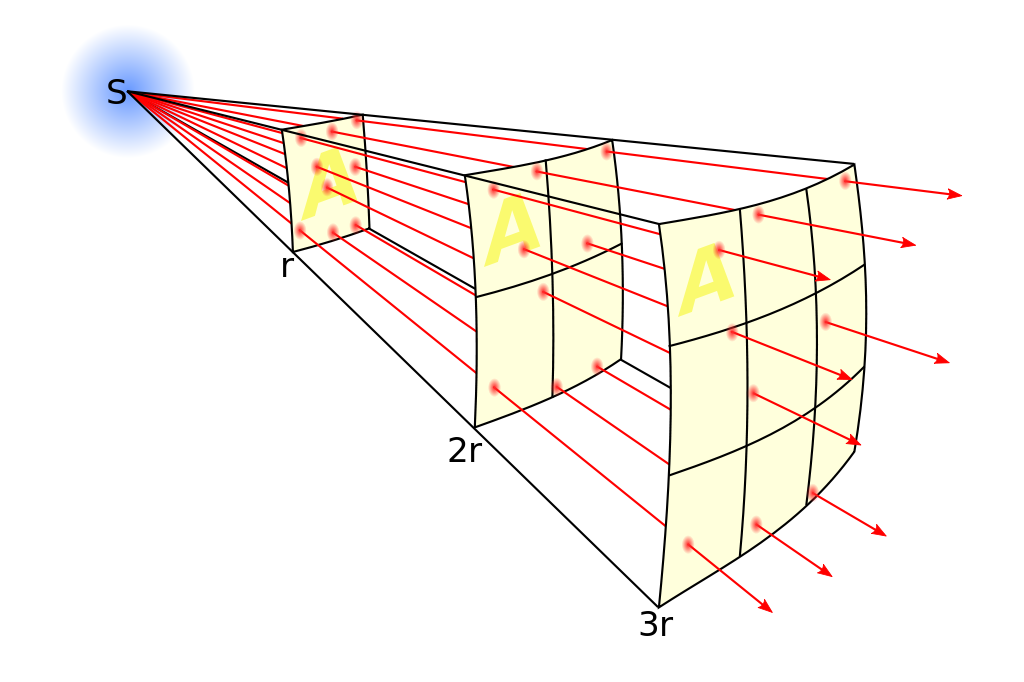
\includegraphics[width=0.4\textwidth]{imagenes/inversesquare.png}
    \caption{La potencia total en cualquier esfera tiene que ser la misma. \footfullcite{inversesquare}}
  \end{figure}
\end{frame}
%--- Next Frame ---%

\begin{frame}{Densidad de potencia}
  \begin{block}{Definición}
    Definimos la \emph{densidad de potencia} como la cantidad de energía electromagnética que atraviesa una superficie de área A en un determinado tiempo
    \begin{equation}
      p = \frac{\Delta E}{\Delta t A}
    \end{equation}
  \end{block}\pause
  \begin{block}{Observación}
  \begin{itemize}[<+->]
    \item A esta magnitud se la suele llamar \emph{irradiancia} en teledetección.
    \item $[E_\lambda] = W m^{-2} \mu m^{-1}$
  \end{itemize}
  \end{block}
\end{frame}
%--- Next Frame ---%

\begin{frame}{Irradiancia espectral}
  Por ahora venimos trabajando con la densidad de potencia total. Pero uno puede preguntarse cuanta energía llegar de cada longitud de onda en el sol.
  \begin{figure}
    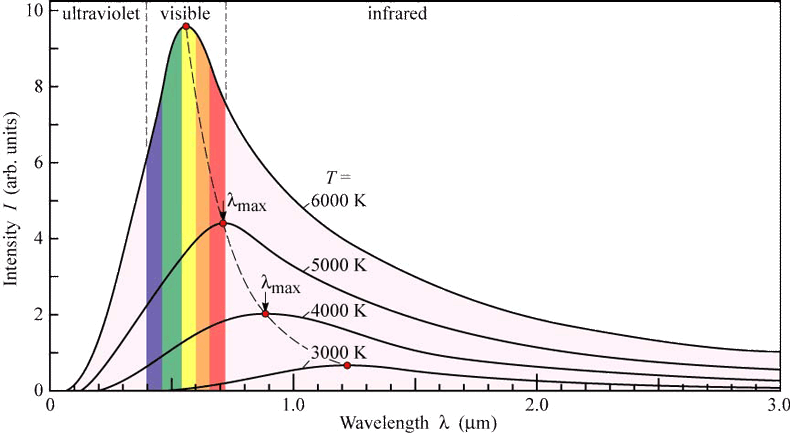
\includegraphics[width=0.8\textwidth]{imagenes/black-body-radiation-curves.png}
    \caption{Curva de radiancia de un cuerpo negro.}
  \end{figure}
\end{frame}
%--- Next Frame ---%

\begin{frame}{Irradiancia espectral}
  \begin{block}{Radiación de cuerpo negro}
    Para un cuerpo negro ideal
    \begin{equation}
      B(\lambda,T) = \frac{2hc^2}{\lambda^5}\frac{1}{e^{\frac{hc}{\lambda k_B T}}-1}
    \end{equation}
  \end{block}
\end{frame}
%--- Next Frame ---%

\begin{frame}{Irradiancia espectral}
  Si miramos ahora lo que llega a la tierra.
  \begin{figure}
    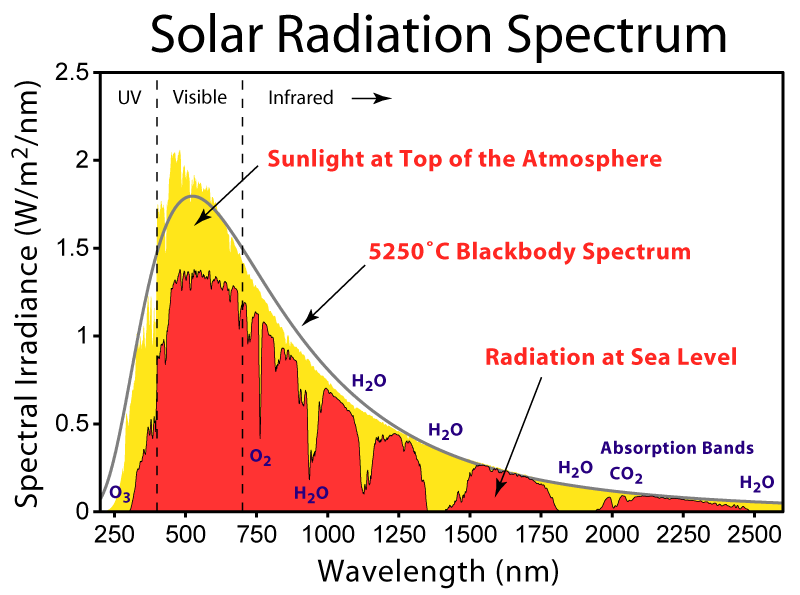
\includegraphics[width=0.6\textwidth]{imagenes/solar_spectrum.png}
    \caption{Irradiancia solar a tope de la atmósfera.\footfullcite{solar_spectrum}}
  \end{figure}
\end{frame}
%--- Next Frame ---%

\begin{frame}{Irradiancia espectral}
  \begin{exampleblock}{Valores de irradiancia espectral}
    En $[E_{0,i}] = \frac{W}{m^2 \mu m}$
    \begin{figure}
      \begin{tabular}{l c c c}
          Banda & ETM+  & TM    &  OLI \\
          Azul     & 1970  & 1954  & 1925 \\
          Verde     & 1843  & 1826  & 1826 \\
          Rojo     & 1555  & 1558  & 1574 \\
          NIR     & 1047  & 1047  & 955  \\
          SWIR1     & 227.1 & 217.2 & 242 \\
          SWIR2     & 80.53 & 80.29 & 82.5\\
      \end{tabular}
    \end{figure}
  \end{exampleblock}
\end{frame}
%--- Next Frame ---%

\begin{frame}{Irradiancia espectral}
  \begin{block}{Definición}
    Llamamos irradiancia espectral a la distribución de irradiancia en función de la longitud de onda.
  \end{block}
\end{frame}
%--- Next Frame ---%

\begin{frame}{Radiancia}
  El último paso será ver como ver como se comporta la irradiancia en función del ángulo.
  \begin{figure}
    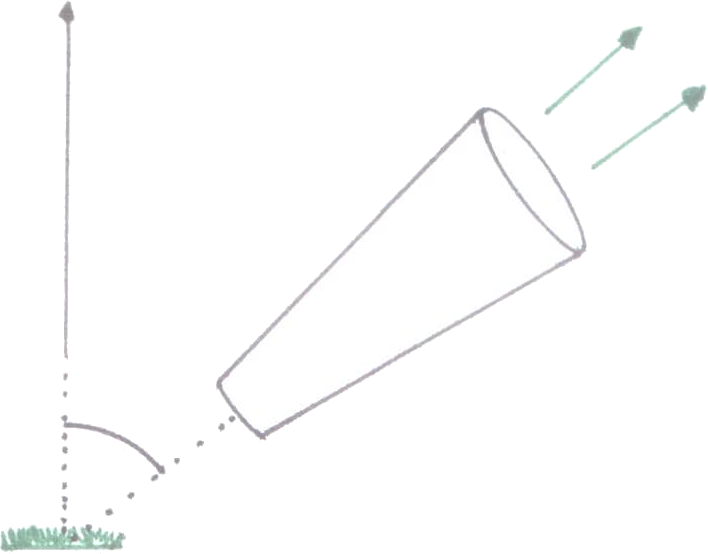
\includegraphics[width=0.4\textwidth]{imagenes/radiancia.png}
    \caption{Cono de radiación.}
  \end{figure}
\end{frame}
%--- Next Frame ---%

\begin{frame}{Radiancia}
  \begin{block}{Definición}
    La radiancia será la irradiancia por unidad de ángulo solido
    \begin{equation}
      L = \frac{p}{\Delta \Omega \cos\theta_z}
    \end{equation}
  \end{block}
\end{frame}
%--- Next Frame ---%

\begin{frame}{Radiancia}
  \begin{itemize}[<+>]
    \item La irradiancia será lo que medirán los sensores.
    \item Depende del ángulo.
    \item Al igual que la irradiancia tiene nos interesara su dependencia espectral.
    \item $[L_\lambda] = W m^{-2} sr^{-1} \mu m^{-1}$
  \end{itemize}
\end{frame}
%--- Next Frame ---%

\begin{frame}{Radiancia}
  \begin{block}{Definición}
    Llamaremos \emph{radiancia espectral} a la magnitud $L_\lambda$ tal que
    \begin{equation}
      dE = L_{\lambda}(\theta,\phi) \cos(\theta) d\Omega dA dt d\lambda
    \end{equation}
  \end{block}
\end{frame}
%--- Next Frame ---%

\begin{frame}{Reflectancia}
  La radiancia no es una buena característica para definir a un cuerpo.
  \begin{exampleblock}{Ejemplo}
  \begin{figure}
    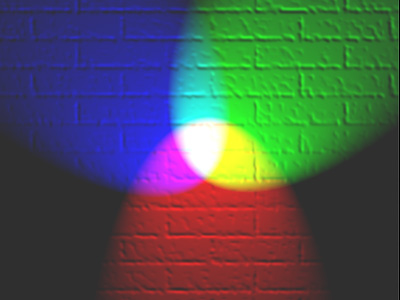
\includegraphics[width=0.4\textwidth]{imagenes/RGBillumination.png}
    \caption{Hojas bajo distintas iluminaciones.\footfullcite{RGBillumination}}
  \end{figure}
  \end{exampleblock}

\end{frame}
%--- Next Frame ---%

\section{Firmas espectrales}
\begin{frame}{Reflectancia}
  Queremos calcular el cociente de la radiancia saliente de una cobertura sobre la radiancia incidente. \pause
  \begin{block}{Definición}
    Definimos la \emph{BRDF} (espectral bidirectional reflectance distribution function) como:
    \begin{equation}
          f(\theta_i, \phi_i, \theta_r, \phi_r) = \frac{dL(\theta_i, \phi_i, \theta_r, \phi_r)}{dE(\theta_i, \phi_i)}
    \end{equation}
  \end{block}
\end{frame}
%--- Next Frame ---%

\begin{frame}{Reflectancia}
  \begin{block}{Definición}
    Definimos la reflectancia direccional como:
    \begin{equation}
     R(\theta_i, \phi_i, \theta_r, \phi_r) = \frac{\pi L(\theta_i, \phi_i, \theta_r, \phi_r)}{\cos(\theta_i) E_0} = \pi f(\theta_i, \phi_i, \theta_r, \phi_r)
    \end{equation}
    Donde $\theta$ y $\phi$ son los ángulos zenitales y azimutales respectivamente.
  \end{block}
\end{frame}
%--- Next Frame ---%

\begin{frame}{Reflectancia direccional}
  \begin{exampleblock}{Ejemplo}
    \begin{figure}
      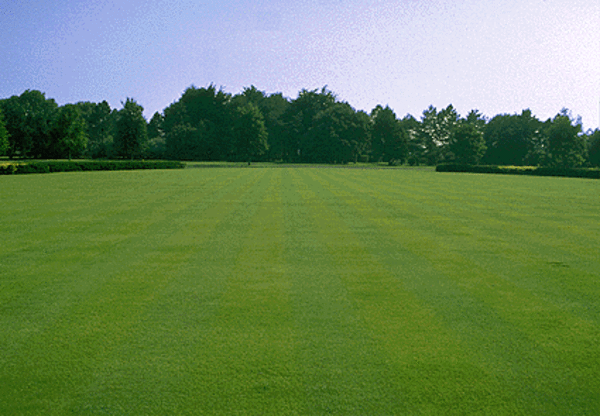
\includegraphics[width=0.6\textwidth]{imagenes/grass.png}
      \caption{Un parque.\footfullcite{grass}}
    \end{figure}
  \end{exampleblock}
\end{frame}

\begin{frame}{Reflectancia direccional}
  \begin{exampleblock}{Ejemplo}
    \begin{figure}
      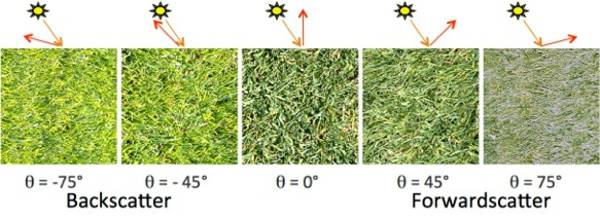
\includegraphics[width=0.6\textwidth]{imagenes/grass2.png}
      \caption{Pasto bajo distintas iluminaciones.\footfullcite{grass}}
    \end{figure}
  \end{exampleblock}
\end{frame}

%--- Next Frame ---%
\begin{frame}{Reflectancia direccional}
  \begin{exampleblock}{Ejemplo}
    \begin{figure}
      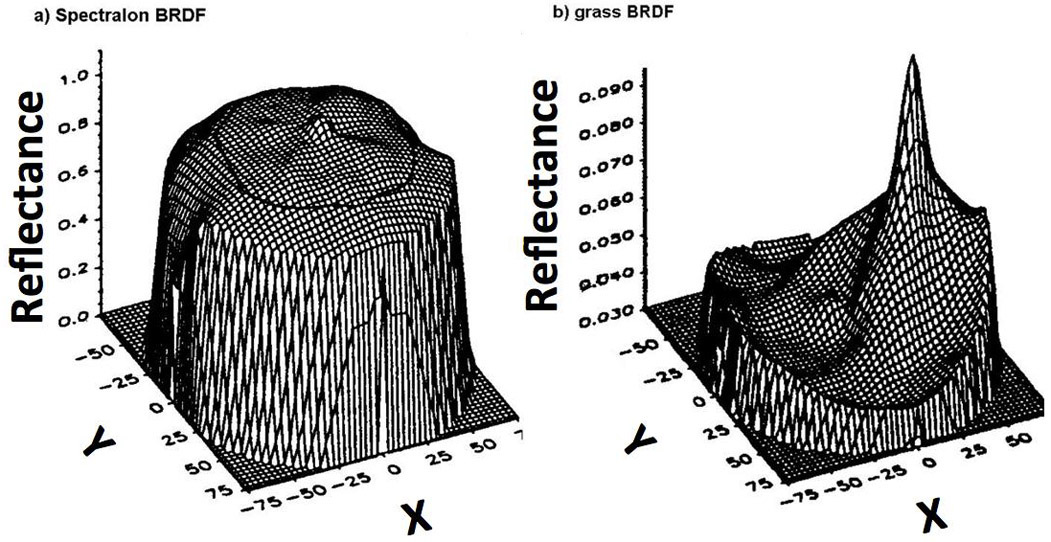
\includegraphics[width=0.6\textwidth]{imagenes/grass_brdf.png}
      \caption{Reflectancia del pasto en función del ángulo zenital y asimutal.\footfullcite{clark2014passive}}
    \end{figure}
  \end{exampleblock}
\end{frame}
%--- Next Frame ---%


%--- Next Frame ---%
\begin{frame}{Reflectancia direccional}
  \begin{figure}
    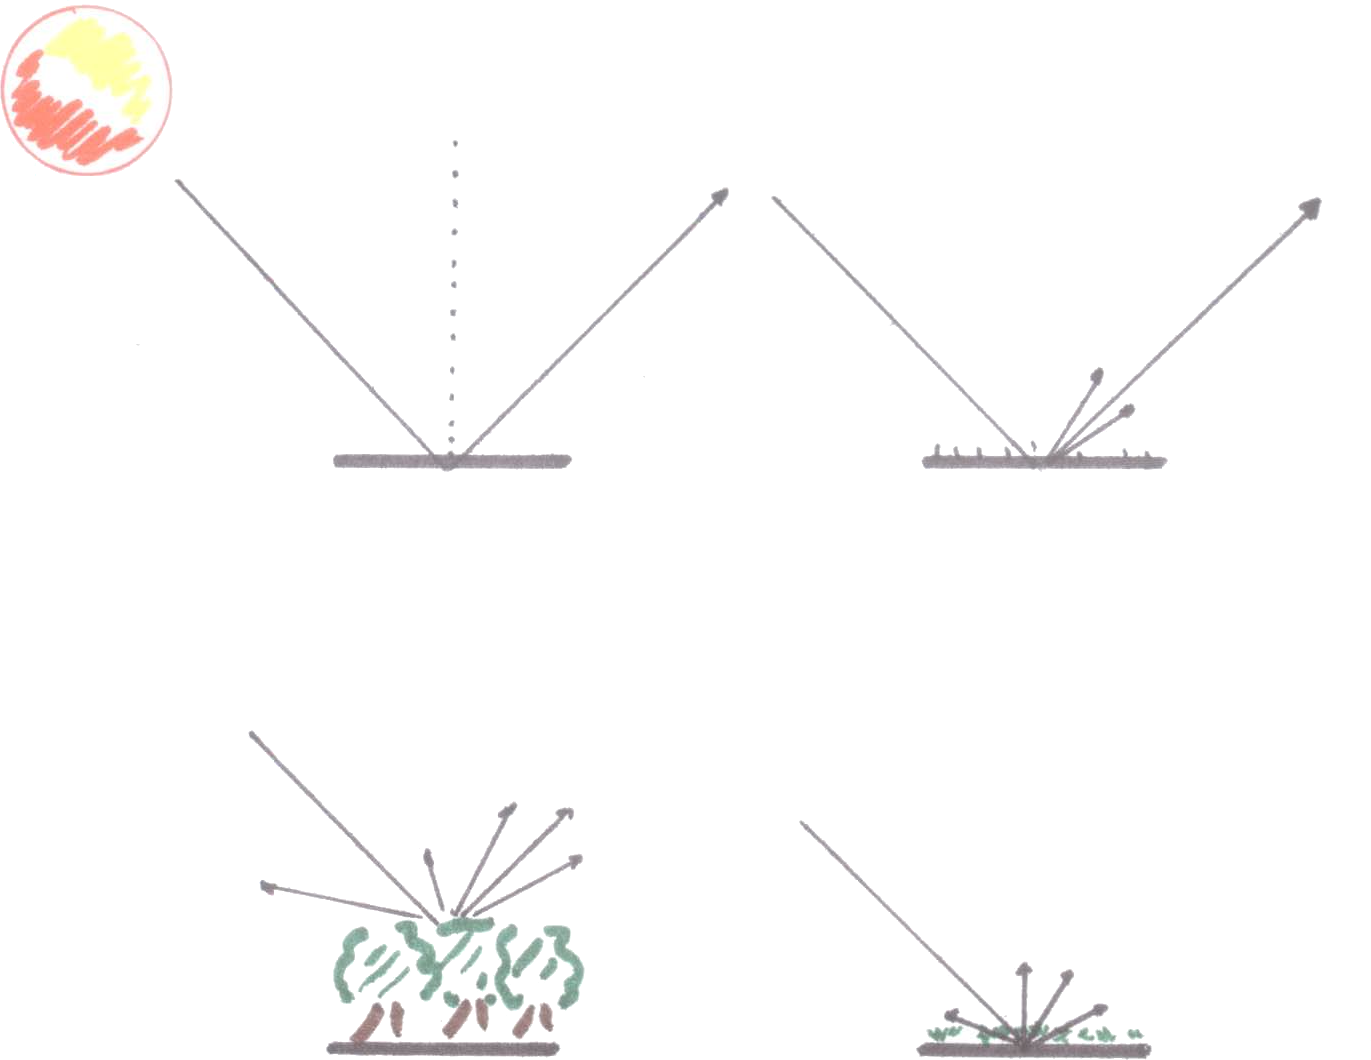
\includegraphics[width=0.6\textwidth]{imagenes/reflectancias.png}
    \caption{En general podemos clasificar la reflectancia en función de que tan fuertemente depende del ángulo.}
  \end{figure}
\end{frame}
%--- Next Frame ---%

\begin{frame}{Aproximaciones}
  \begin{block}{Definición}
    Hablamos de la aproximación \emph{especular} cuando la reflectancia es una delta del ángulo.
  \end{block}\pause
  \begin{block}{Definición}
    Hablamos de la aproximación \emph{lambertiana} cuando la reflectancia no depende del ángulo.
  \end{block}
\end{frame}

\begin{frame}{Aproximaciones}
  \begin{alertblock}{Importante}
    En el curso vamos a trabajar en la aproximación Lambertiana. Esto es solo una aproximación que simplifica y mucho el problema.
  \end{alertblock}
\end{frame}
%--- Next Frame ---%

\begin{frame}{Reflectancia}
  \begin{block}{Definición}
    En la aproximación lambertiana defininos la \emph{reflectancia} como
    \begin{equation}
      \rho = \frac{\pi L}{\cos \theta_z E_0}
    \end{equation}
  \end{block}
\end{frame}

\begin{frame}{Aproximaciones}
  \begin{alertblock}{Importante}
    La reflectancia depende solo de la superficie que estamos mirando.
  \end{alertblock}
\end{frame}
%--- Next Frame ---%

\begin{frame}{Firma espectral}
  Si ahora pensamos como depende la reflectancia de la longitud de onda podemos definir
  \begin{block}{Definición}
    Llamamos firma espectral a la función de la reflectancia como función de la longitud de onda, $\rho_\lambda$.
  \end{block}\pause
  Veamos algunos ejemplos y de por que sirven para describir a las coberturas.\pause
  \begin{itemize}
    \item Vegetación
    \item Suelo
    \item Agua
  \end{itemize}
\end{frame}


\begin{frame}{Firma espectral - vegetación}
  \begin{figure}
  \
  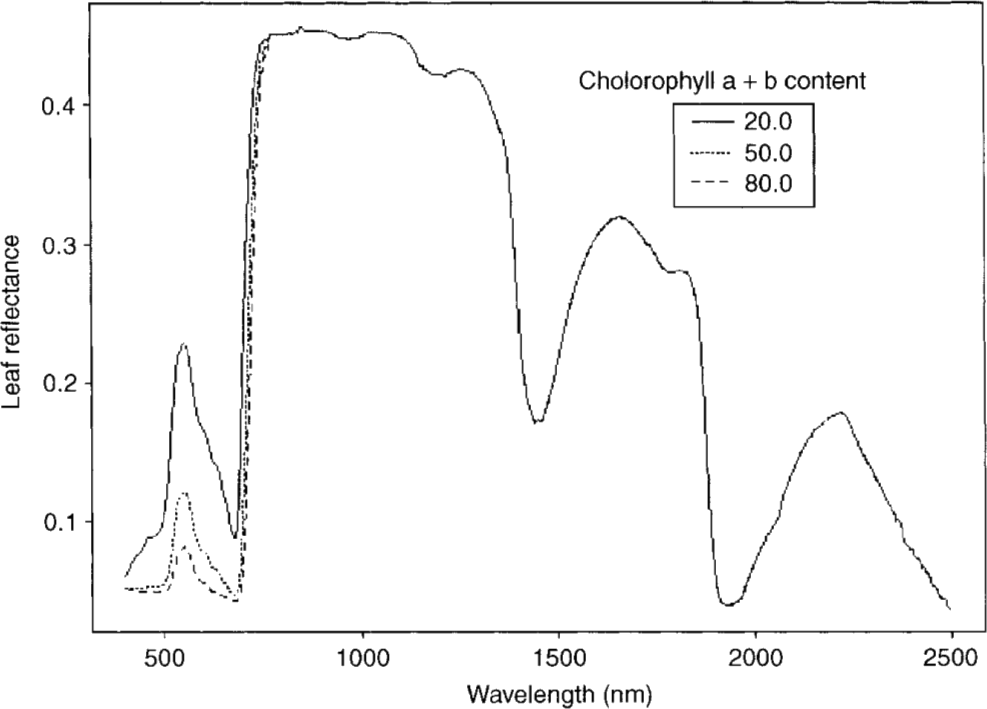
\includegraphics[width=0.8\textwidth]{imagenes/clorovar.png}
  \caption{Variaciones de la firma espectral con el contenido de clorofila.\footfullcite{liang2005quantitative}}
  \end{figure}
\end{frame}
%--- Next Frame ---%

\begin{frame}{Firma espectral - vegetación}
  \begin{figure}

  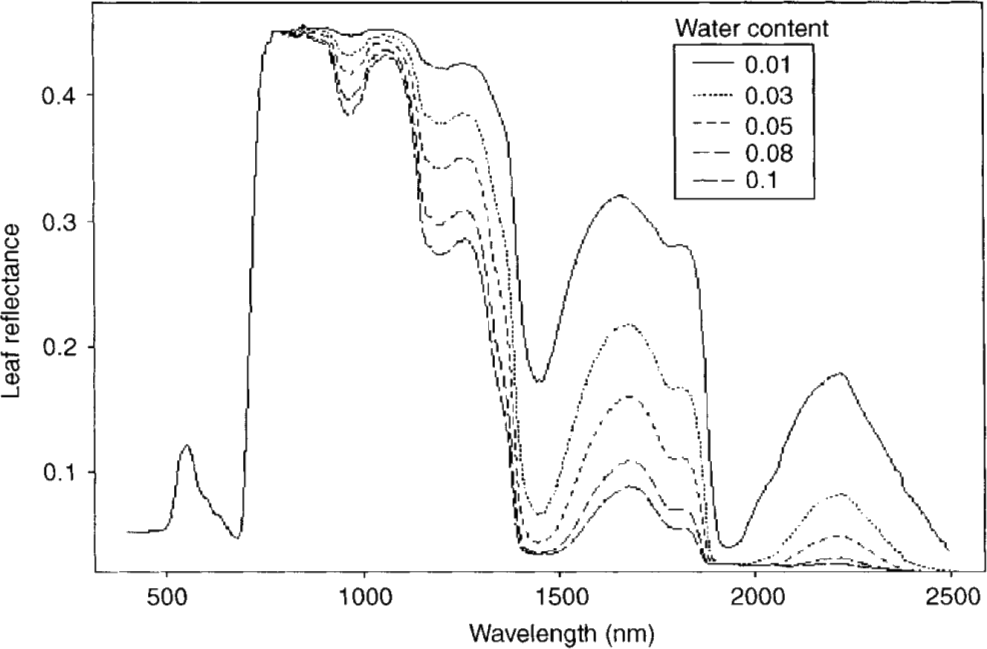
\includegraphics[width=0.8\textwidth]{imagenes/vwvar.png}
  \caption{Variaciones de la firma espectral con el contenido de agua.\footfullcite{liang2005quantitative}}
  \end{figure}
\end{frame}
%--- Next Frame ---%

\begin{frame}{Firma espectral - vegetación}
  \begin{figure}

  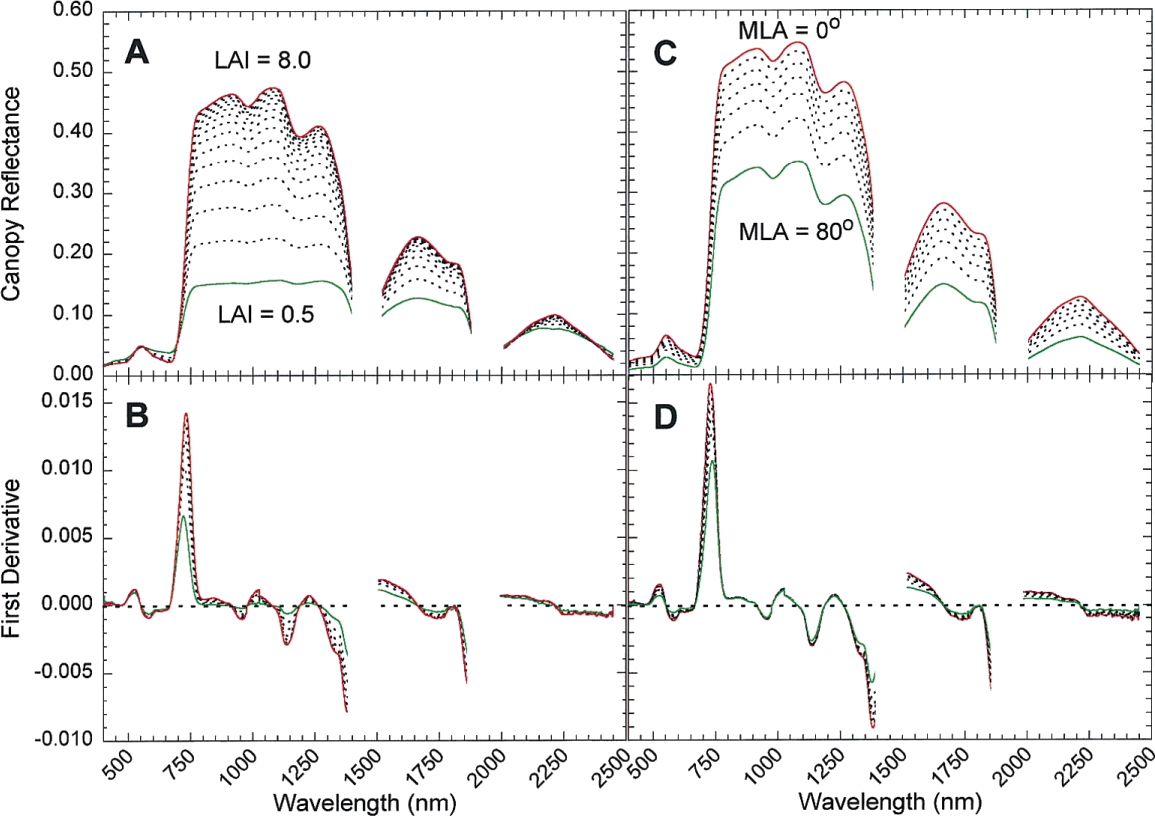
\includegraphics[width=0.8\textwidth]{imagenes/leafvar.png}
  \caption{Variaciones de la firma espectral con el área foliar.\footfullcite{asner1998biophysical}}
  \end{figure}
\end{frame}
%--- Next Frame ---%

\begin{frame}{Firma espectral - vegetación}
    \begin{figure}

    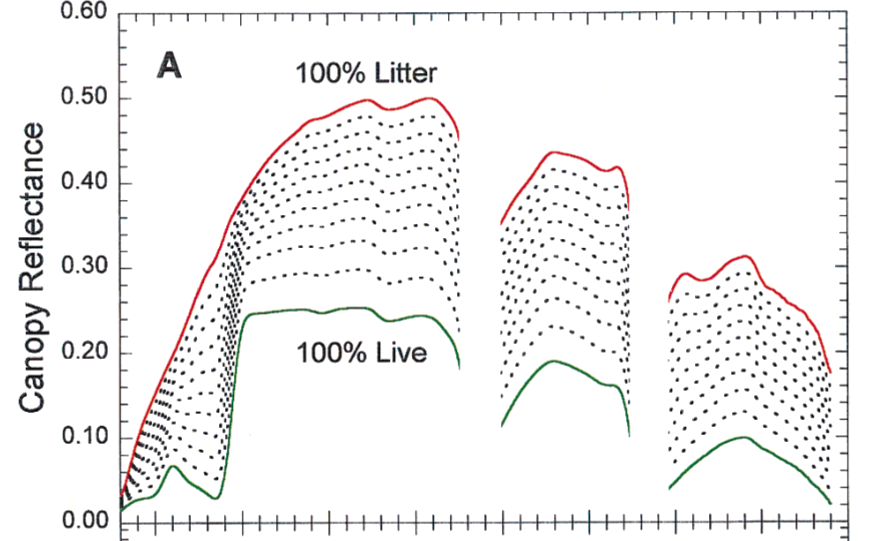
\includegraphics[width=0.8\textwidth]{imagenes/vivomuerto.png}
    \caption{Firma espectral de la vegetación en diferentes estados.\footfullcite{asner1998biophysical}}
    \end{figure}
\end{frame}
%--- Next Frame ---%

\begin{frame}{Firma espectral - suelo}
    \begin{figure}

    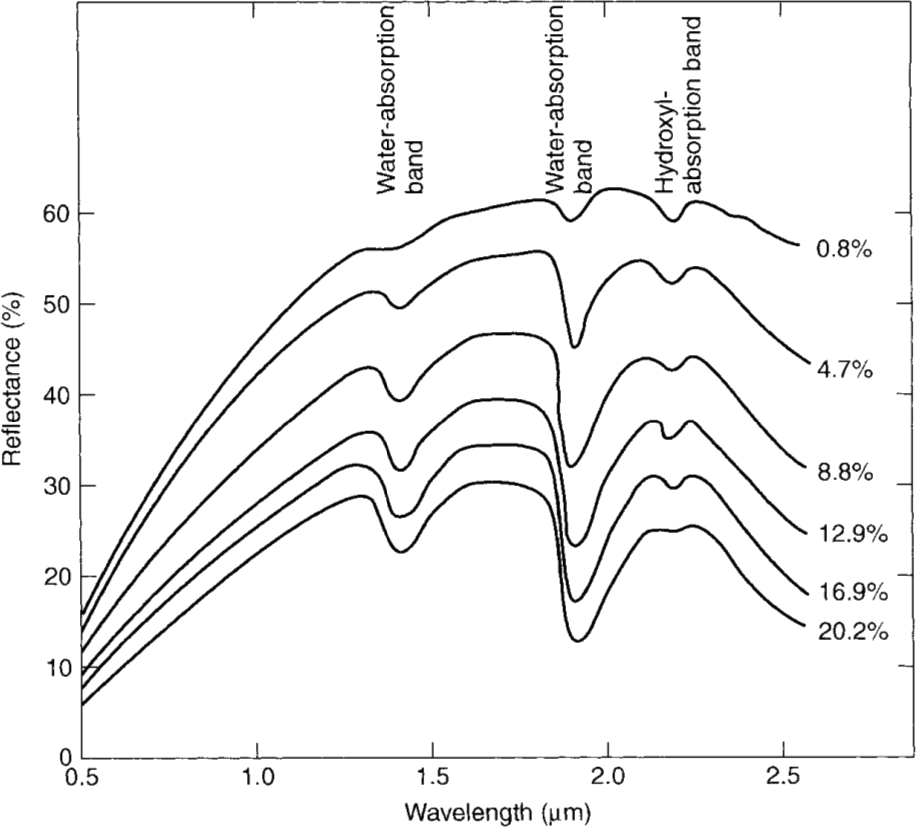
\includegraphics[width=0.6\textwidth]{imagenes/soilvar.png}
    \caption{Firma espectral del suelo con distintos contenidos de humedad.\footfullcite{liang2005quantitative}}
    \end{figure}
\end{frame}
%--- Next Frame ---%

\begin{frame}{Firma espectral - agua}
    \begin{figure}

    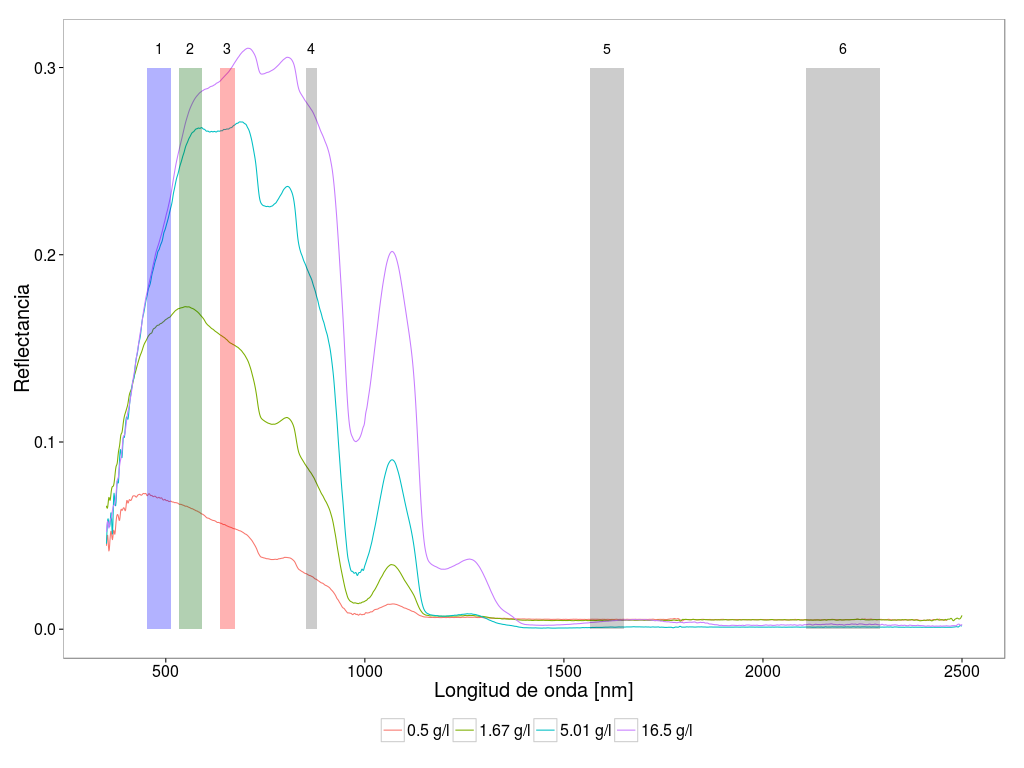
\includegraphics[width=0.8\textwidth]{imagenes/waterm.png}
    \caption{Firma espectral de agua con distinto contenido de arcilla disuelta.\footfullcite{clark2007usgs}}
    \end{figure}
\end{frame}
%--- Next Frame ---%

\begin{frame}{Firma espectral - agua}
    \begin{figure}
    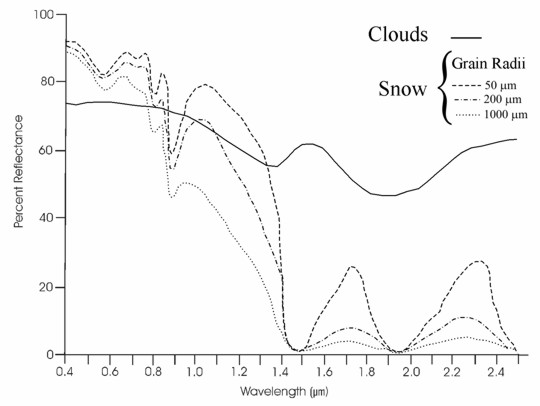
\includegraphics[width=0.8\textwidth]{imagenes/snow.png}
    \caption{Firma espectral de agua en distintos estados de agregación.\footfullcite{snow}}
    \end{figure}
\end{frame}
%--- Next Frame ---%

\section{Espacio espectral}
\begin{frame}{Discretización de la firma espectral}
  Hasta ahora la firma espectral es continua. Estudiemos que le pasa cuando el sensor la mide.
\end{frame}
%--- Next Frame ---%

\begin{frame}{Respuesta espectral}
  \begin{block}{Definición}
    Hablamos de la \emph{respuesta espectral de un sensor} cuando hablamos de como mide la luz que le llega al mismo en el dominio espectral.
  \end{block}
\end{frame}
%--- Next Frame ---%

\begin{frame}[t]{Respuesta espectral}
    \begin{exampleblock}{Ejemplo}
        \begin{figure}
            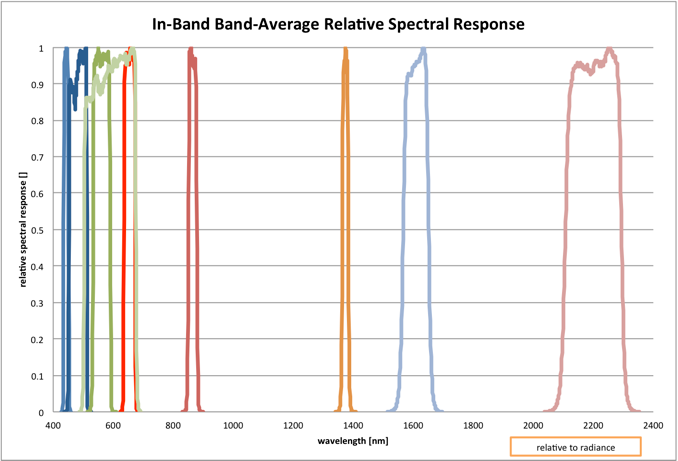
\includegraphics[width=0.67\textwidth]{imagenes/AllBandsRSR.png}
            \caption{Respuestas espectrales de las bandas de Landsat 8.\footfullcite{barsi2014spectral}}
        \end{figure}
    \end{exampleblock}
\end{frame}
%--- Next Frame ---%

\begin{frame}{Respuesta espectral}
  Matematicamente, cuando un sensor mide la luz reflejada por un parche en el suelo esta haciendo un promedio pesado. Es decir:
  \begin{block}{Definición}
    El valor de brillo tomado por un sensor esta dado por
    \begin{equation}
        L_{j} =\frac{\int s_j(\lambda) L_\lambda d\lambda}{\int s_j(\lambda) d\lambda}.
    \end{equation}
  \end{block}
  esto para cada una de las N bandas de un sensor.
\end{frame}
%--- Next Frame ---%

\begin{frame}{Respuesta espectral}
  \begin{block}{Observación}
  \begin{itemize}
  \item El centro y el semi-ancho de un filtro nos permiten definir el centro de la banda y la correspondiente resolución espectral de la misma.
  \item En conclusión, al terminar el día la firma espectral queda discretizada según el número de bandas que usemos.
  \end{itemize}
  \end{block}
\end{frame}
%--- Next Frame ---%

\begin{frame}{Pixeles}
  Cada píxel va a tener asociado distintos valores de brillo, uno por banda de adquisición. \pause
  \begin{block}{Definición}
    Hablamos de un vector píxel al vector construido como
    \begin{equation}
      p = (\rho_1, \ldots ,\rho_N)
    \end{equation}
  \end{block}
\end{frame}
%--- Next Frame ---%

\begin{frame}{Píxeles - vectores}
  \begin{exampleblock}{Ejemplo}
    \begin{figure}
      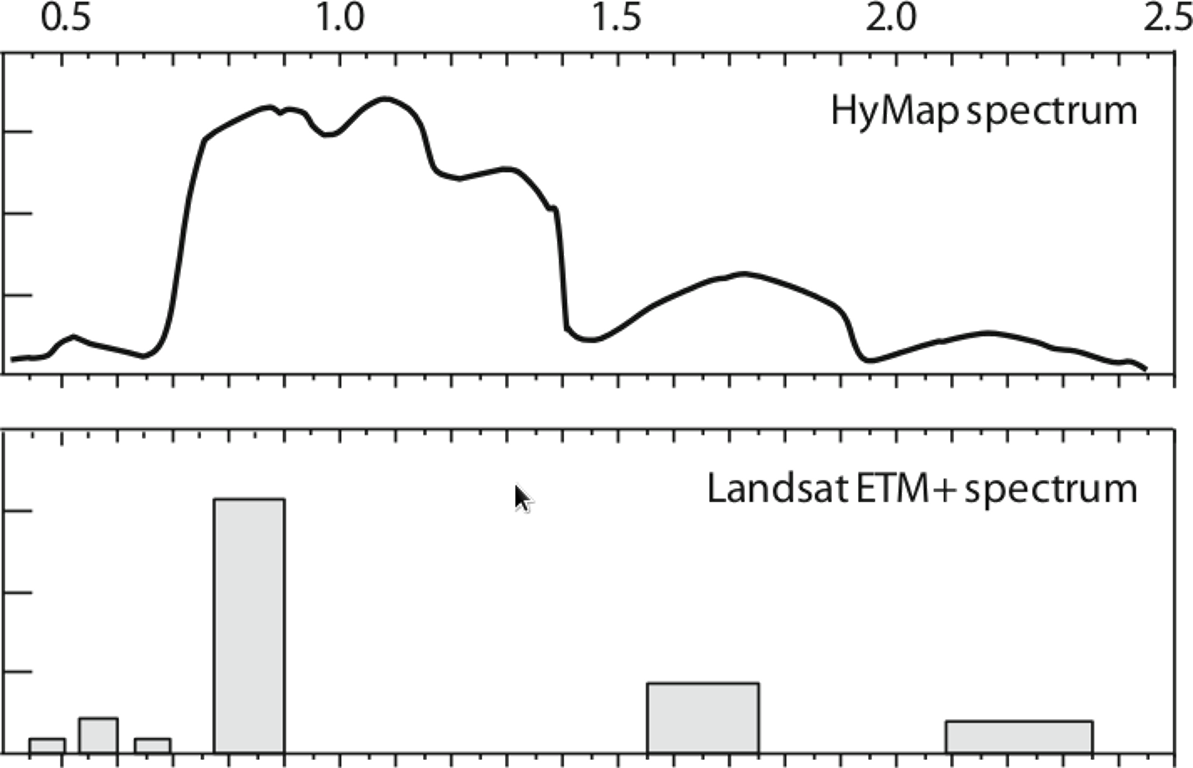
\includegraphics[width=0.6\textwidth]{imagenes/elandsat.png}
    \end{figure}
  \end{exampleblock}
\end{frame}
%--- Next Frame ---%

\begin{frame}{Vectores}
  \begin{exampleblock}{Ejemplo}
    \begin{figure}
      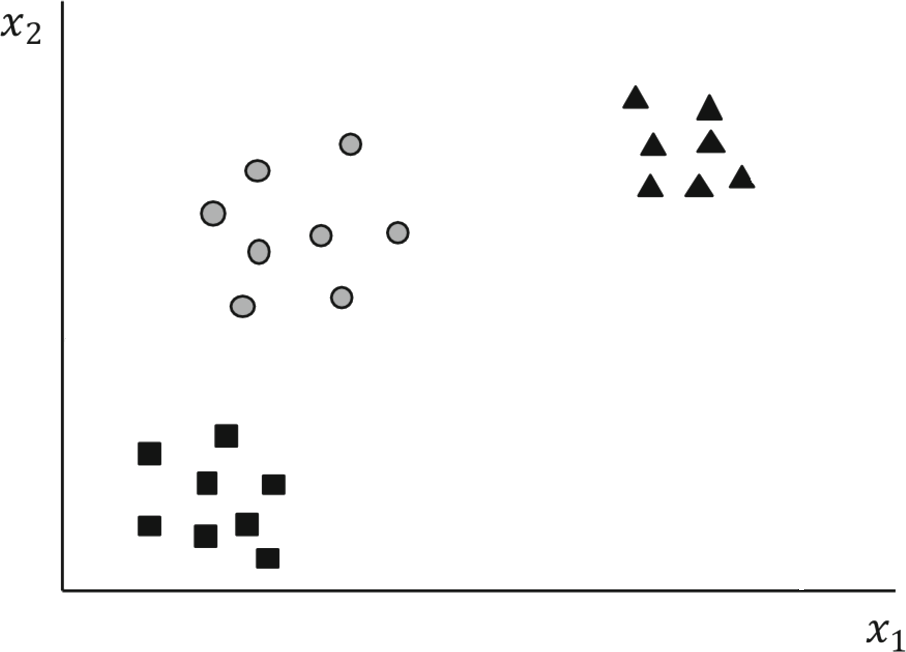
\includegraphics[width=0.5\textwidth]{imagenes/vector-3.png}
      \caption{Espacio espectral con 3 componentes y dos bandas. \footfullcite{richards2013remote}}
    \end{figure}
  \end{exampleblock}
\end{frame}
%--- Next Frame ---%

\begin{frame}{Espacio espectral}
  \begin{block}{Definición}
    Llamaremos \emph{espacio espectral} al espacio donde viven todos los vectores píxeles.
  \end{block}
\end{frame}
%--- Next Frame ---%

\section{Práctica}

\begin{frame}{Práctica}
  \begin{exampleblock}{Actividades prácticas de la primera clase}
    \begin{enumerate}
      \item Abrir imágenes Landsat 8 y familiarizarse con el SoPI.
      \item Digitalizar coberturas uniformes dentro de la imagen.
      \item Extraer la firma espectral de las coberturas digitalizadas.
    \end{enumerate}
  \end{exampleblock}
\end{frame}
%--- Next Frame ---%

\end{document}
